\section{Experimentació}

Hem realitzat una anàlisi experimental per avaluar l'evolució del temps de planificació en funció de la mida del problema. L'objectiu és minimitzar els costos d'assignació mentre es gestionen les restriccions del problema. Hem dissenyat tres experiments que analitzen diferents dimensions del creixement del problema.

\subsection{Experiment 1}

Aquest experiment avalua l'impacte del \textbf{creixement del nombre d’habitacions} mantenint constant el nombre de reserves.

\subsubsection{Configuració}
\begin{itemize}
    \item Nombre de mostres: 9
    \item Habitacions: de 4 a 12 (creixent)
    \item Reserves: 4 (constant)
\end{itemize}

\subsubsection{Resultats}

\begin{table}[h]
\centering
\begin{tabular}{|c|c|c|c|c|c|}
\hline
Problema & Nombre Estats & Nombre Fets & Nombre Habitacions & Nombre Reserves & Temps (s) \\
\hline
1 & 53 & 169 & 4 & 4 & 0.16 \\
2 & 193 & 279 & 5 & 4 & 0.16 \\
3 & 239 & 308 & 6 & 4 & 0.16 \\
4 & 339 & 387 & 7 & 4 & 0.16 \\
5 & 1795 & 418 & 8 & 4 & 0.46 \\
6 & 731 & 421 & 9 & 4 & 0.31 \\
7 & 1039 & 524 & 10 & 4 & 0.31 \\
8 & 1439 & 549 & 11 & 4 & 0.46 \\
9 & 1271 & 592 & 12 & 4 & 0.62 \\
\hline
\end{tabular}
\caption{Resultats Experiment 1}
\end{table}

Els resultats mostren un creixement moderat del temps de planificació. Es detecta un increment significatiu en el nombre d'estats explorats, passant de 53 a 1795 estats. Atribuïm el creixement i decreixement del temps d'execució a que els problemes són generats aleatòriament, i per casualitat un problema pot ser més difícil que un altre, per exemple si hi han reserves que ocupen molts dies i són fàcils de descartar

\begin{figure}[h]
\centering
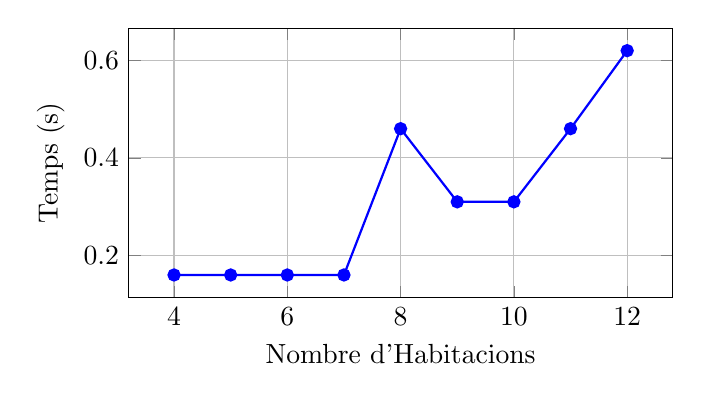
\begin{tikzpicture}
\begin{axis}[
    xlabel={Nombre d'Habitacions},
    ylabel={Temps (s)},
    width=0.7\textwidth,
    height=5cm,
    grid=major,
    legend pos=north west,
    ymajorgrids=true,
    xmajorgrids=true
]
\addplot[color=blue,mark=*,thick] coordinates {
    (4,0.16) (5,0.16) (6,0.16) (7,0.16) (8,0.46) (9,0.31) (10,0.31) (11,0.46) (12,0.62)
};
\end{axis}
\end{tikzpicture}
\caption{Evolució del temps de planificació amb creixement d'habitacions}
\end{figure}

\FloatBarrier
\subsection{Experiment 2}

El segon experiment analitza l'efecte del \textbf{creixement del nombre de reserves} mantenint constant el nombre d'habitacions.

\subsubsection{Configuració}
\begin{itemize}
    \item Nombre de mostres: 9
    \item Habitacions: 4 (constant)
    \item Reserves: de 4 a 12 (creixent)
\end{itemize}

\subsubsection{Resultats} 

\begin{table}[h]
\centering

\begin{tabular}{|c|c|c|c|c|c|}
\hline
Problema & Nombre Estats & Nombre Fets & Nombre Habitacions & Nombre Reserves & Temps (s) \\
\hline
1 & 53 & 169 & 4 & 4 & 0.16 \\
2 & 346 & 224 & 4 & 5 & 0.32 \\
3 & 1692 & 233 & 4 & 6 & 0.46 \\
4 & 1259 & 237 & 4 & 7 & 0.47 \\
5 & 53313 & 277 & 4 & 8 & 790.95 \\
6 & 251587 & 263 & 4 & 9 & 16313.28 \\
7 & 55116 & 260 & 4 & 10 & 431.25 \\
8 & -- & -- & 4 & 11 & inf \\
9 & 245691 & 297 & 4 & 12 & 10268.28 \\
\hline
\end{tabular}
\caption{Resultats Experiment 2}
\end{table}


Els resultats evidencien un creixement exponencial del temps de planificació. Amb 4 reserves el temps és de 0.16s, però amb 9 reserves arriba a aproximadament 4.5 hores. El problema amb 11 reserves no va trobar solució, va petar la memòria abans d'acabar. 

\begin{figure}[h]
\centering
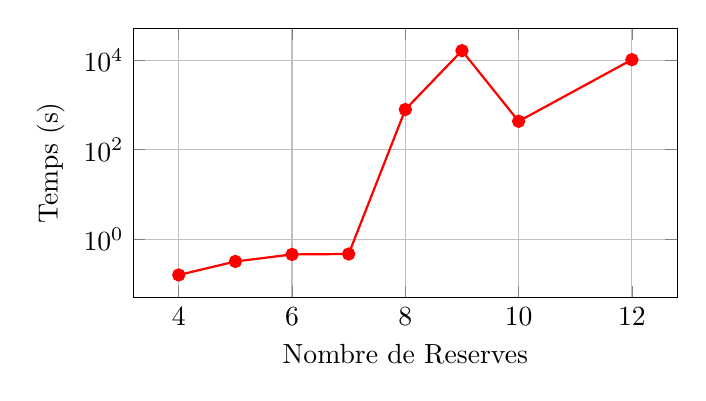
\begin{tikzpicture}
\begin{axis}[
    xlabel={Nombre de Reserves},
    ylabel={Temps (s)},
    width=0.7\textwidth,
    height=5cm,
    grid=major,
    legend pos=north west,
    ymode=log,
    ymajorgrids=true,
    xmajorgrids=true,
    log basis y=10
]
\addplot[color=red,mark=*,thick] coordinates {
    (4,0.16) (5,0.32) (6,0.46) (7,0.47) (8,790.95) (9,16313.28) (10,431.25) (12,10268.28)
};
\end{axis}
\end{tikzpicture}
\caption{Evolució del temps de planificació amb creixement de reserves (escala logarítmica)}
\end{figure}

\FloatBarrier
\subsection{Comparació entre els experiments 1 i 2}

Com és d'esperar, incrementar el nombre d'habitacions com en l'experiment 1, no és un problema per el planificador, el creixement és quasi constant, ara bé, incrementar el nombre de reserves, significa fer moltes mes comprovacions per el mateix nombre d'habitacions, moltes més combinacions possibles que tenen un impacte molt més significatiu en la complexitat computacional. A la figura 3 veiem la comparació entre temps d'execució.

% Comparació temps d'execució
\begin{figure}[h]
\centering
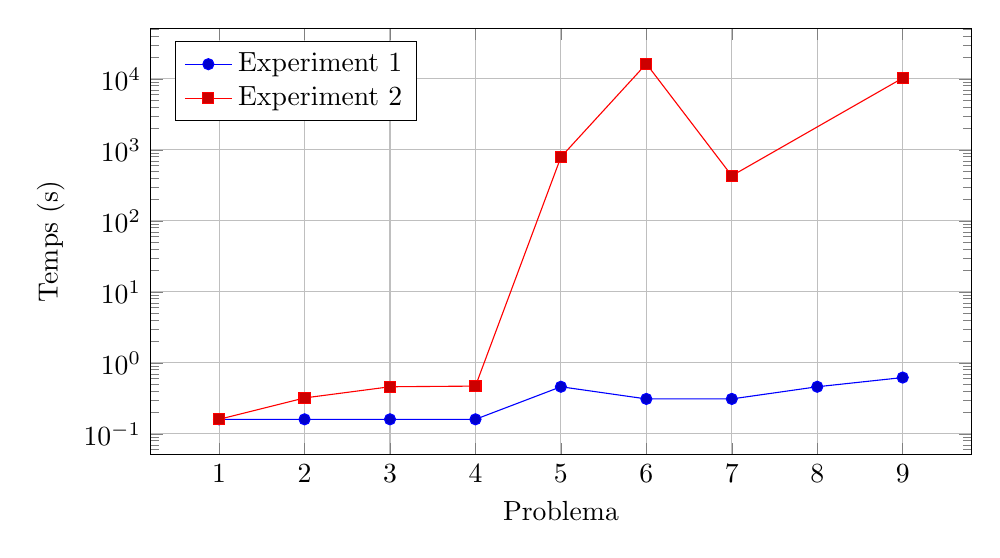
\begin{tikzpicture}
\begin{axis}[
    xlabel={Problema},
    ylabel={Temps (s)},
    legend pos=north west,
    grid=major,
    width=12cm,
    ymode=log,
    height=7cm
]
% Experiment 1
\addplot coordinates {
    (1,0.16) (2,0.16) (3,0.16) (4,0.16)
    (5,0.46) (6,0.31) (7,0.31) (8,0.46) (9,0.62)
};
\addlegendentry{Experiment 1}
% Experiment 2
\addplot coordinates {
    (1,0.16) (2,0.32) (3,0.46) (4,0.47)
    (5,790.95) (6,16313.28) (7,431.25) (9,10268.28)
};
\addlegendentry{Experiment 2}
\end{axis}
\end{tikzpicture}
\caption{Comparació del temps d'execució entre els experiments 1 i 2 (escala logarítmica)}
\end{figure}

Pel que fa al nombre d'estats, veiem que el creixement és semblant, amb un creixement important al cinquè problema i després un creixement més moderat

% Nombre d'estats
\begin{figure}[h]
\centering
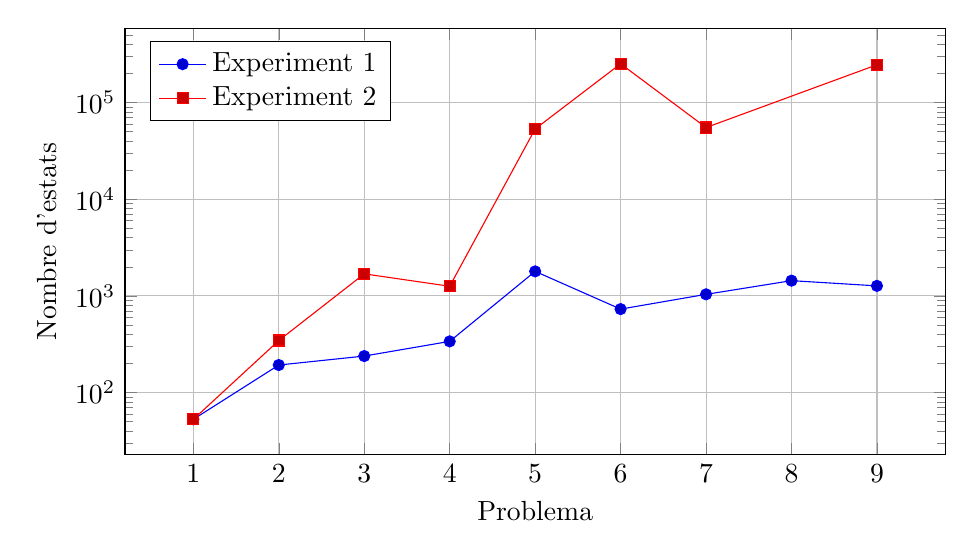
\begin{tikzpicture}
\begin{axis}[
    xlabel={Problema},
    ylabel={Nombre d'estats},
    legend pos=north west,
    grid=major,
    width=12cm,
    ymode=log,
    height=7cm
]
% Experiment 1 - Estats
\addplot coordinates {
    (1,53) (2,193) (3,239) (4,339)
    (5,1795) (6,731) (7,1039) (8,1439) (9,1271)
};
\addlegendentry{Experiment 1}
% Experiment 2 - Estats
\addplot coordinates {
    (1,53) (2,346) (3,1692) (4,1259)
    (5,53313) (6,251587) (7,55116) (9,245691)
};
\addlegendentry{Experiment 2}
\end{axis}
\end{tikzpicture}
\caption{Comparació del nombre d'estats entre Experiment 1 i Experiment 2 (escala logarítmica)}
\end{figure}

I finalment, el nombre de fets també té un creixement semblant, tot i que la quantitat acaba sent molt menor al nombre d'estats o temps d'execució

% Nombre de fets
\begin{figure}[h]
\centering
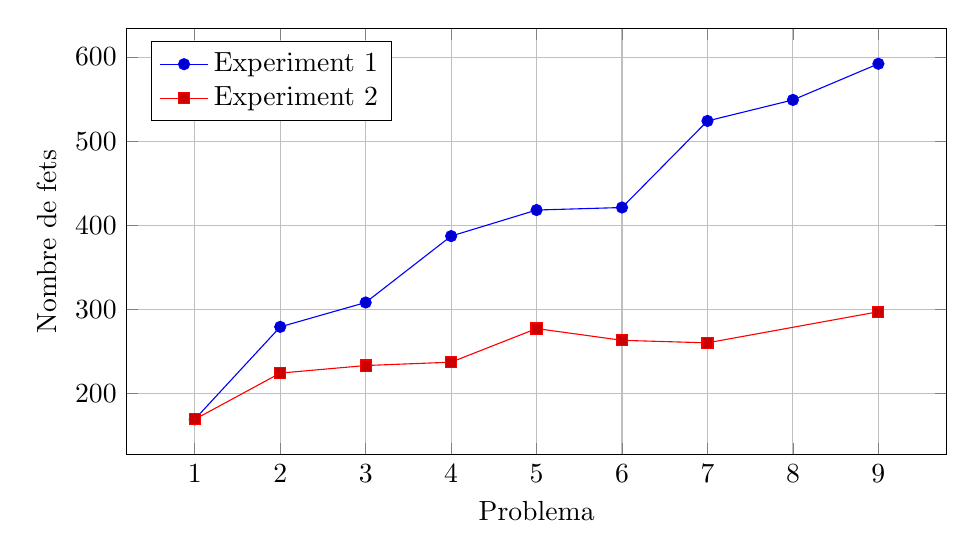
\begin{tikzpicture}
\begin{axis}[
    xlabel={Problema},
    ylabel={Nombre de fets},
    legend pos=north west,
    grid=major,
    width=12cm,
    height=7cm
]
% Experiment 1 - Fets
\addplot coordinates {
    (1,169) (2,279) (3,308) (4,387)
    (5,418) (6,421) (7,524) (8,549) (9,592)
};
\addlegendentry{Experiment 1}
% Experiment 2 - Fets
\addplot coordinates {
    (1,169) (2,224) (3,233) (4,237)
    (5,277) (6,263) (7,260) (9,297)
};
\addlegendentry{Experiment 2}
\end{axis}
\end{tikzpicture}
\caption{Comparació del nombre de fets entre Experiment 1 i Experiment 2}
\end{figure}


\FloatBarrier
\subsection{Experiment 3}

L'últim experiment combina el \textbf{creixement simultani d'habitacions i reserves} per analitzar l'efecte conjunt. 

\subsubsection{Configuració}
\begin{itemize}
    \item Nombre de mostres: 5
    \item Habitacions: de 3 a 7 (creixent)
    \item Reserves: de 4 a 8 (creixent)
\end{itemize}

\subsubsection{Resultats} 

\begin{table}[h]
\centering

\begin{tabular}{|c|c|c|c|c|c|}
\hline
Problema & Nombre Estats & Nombre Fets & Nombre Habitacions & Nombre Reserves & Temps (s) \\
\hline
1 & 54 & 151 & 3 & 4 & 0.00 \\
2 & 408 & 222 & 4 & 5 & 0.16 \\
3 & 614 & 240 & 5 & 6 & 0.00 \\
4 & 54880 & 386 & 6 & 7 & 670.31 \\
5 & 375683 & 442 & 7 & 8 & 46820.47 \\
\hline
\end{tabular}
\caption{Resultats Experiment 3}
\end{table}

Els resultats mostren un creixement exponencial molt pronunciat. El temps passa de valors pràcticament instantanis a aproximadament 13 hores. El nombre d'estats explorats creix moltíssim, arribant a 375683 estats en l'últim problema.

\begin{figure}[h]
\centering
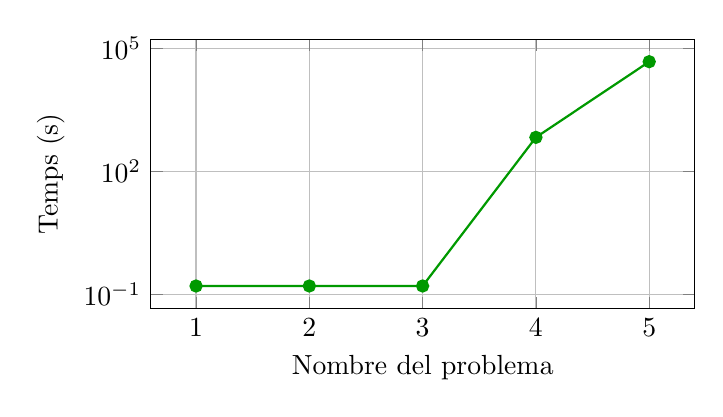
\begin{tikzpicture}
\begin{axis}[
    xlabel={Nombre del problema},
    ylabel={Temps (s)},
    width=0.7\textwidth,
    height=5cm,
    grid=major,
    legend pos=north west,
    ymode=log,
    ymajorgrids=true,
    xmajorgrids=true,
    log basis y=10,
    xtick={1,2,3,4,5},
    xticklabels={1,2,3,4,5}
]
\addplot[color=green!60!black,mark=*,thick] coordinates {
    (1,0.16) (2,0.16) (3,0.16) (4,670.31) (5,46820.47)
};
\end{axis}
\end{tikzpicture}
\caption{Evolució del temps amb creixement simultani (escala logarítmica)}
\end{figure}


